\documentclass{article}
\usepackage[utf8]{inputenc}
\usepackage{lipsum} % Used for tableofcontents
\usepackage[parfill]{parskip} % No indent for a new line
\usepackage[capitalise]{cleveref} % cref
\usepackage{mwe} % used for minipages to show two figures side by side
\usepackage{subcaption}
\usepackage{enumitem}
\usepackage{cite}
\usepackage{graphicx}
\usepackage{float}
\usepackage[margin=1.5in]{geometry}
\graphicspath{{./figures/}}


\title{ACML Homework \\ Music by RNNs}
\author{Ibrahim Hadzic (i6200920), Alexander Reisach (i6197692)}
\date{\today}

\begin{document}
\maketitle

\section{Getting Things Running}
% We adapted the code from \textit{https://github.com/brannondorsey/midi-rnn} to tensorflow 2.1, and ran some experiments with the default settings. As can be seen in \ref{fig:tensorboard_2}, although training loss is steadily decreasing, there is no clear trend visible for the validation performance.

\begin{figure}[h]
    \centering
    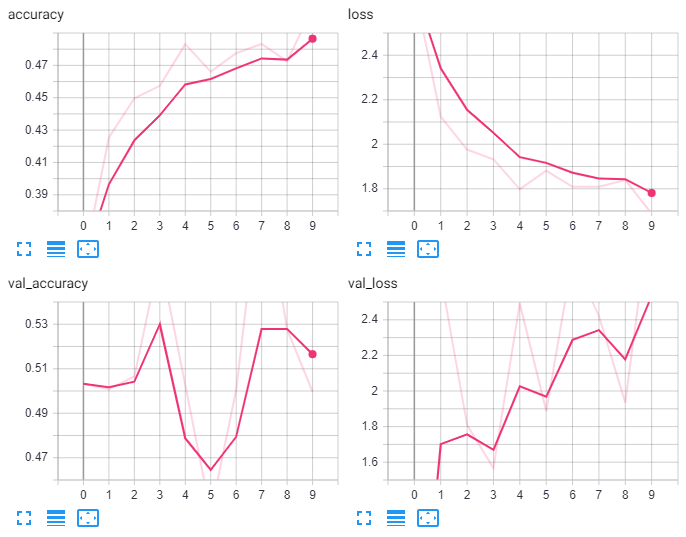
\includegraphics[scale=0.45]{tensorboard_2.png}
    \caption{Tensorboard output for default settings}
    \label{fig:tensorboard_1}
\end{figure}

In order to test different and more computationally intensive settings, we use the Aachen cluster's gpu. We use keras' CuDNNLSTM layers instead of regular LSTM layers to take advantage of the accelerated linear algebra (XLA) optimizations.


\section{Experiments}
Ever since the term "random guessing" has come out of fashion, we have specialized in "principled experimentation" instead, and this project is no exception. Following best practices from the internet (c.f. \ref{fig:good_advice}), we experimented in particular with the following parameters:
\begin{itemize}
    \item number of (LSTM) layers
    \item nodes per (LSTM) layer
    \item input window size
    \item numper of training epochs
\end{itemize}

\begin{figure}[h]
    \centering
    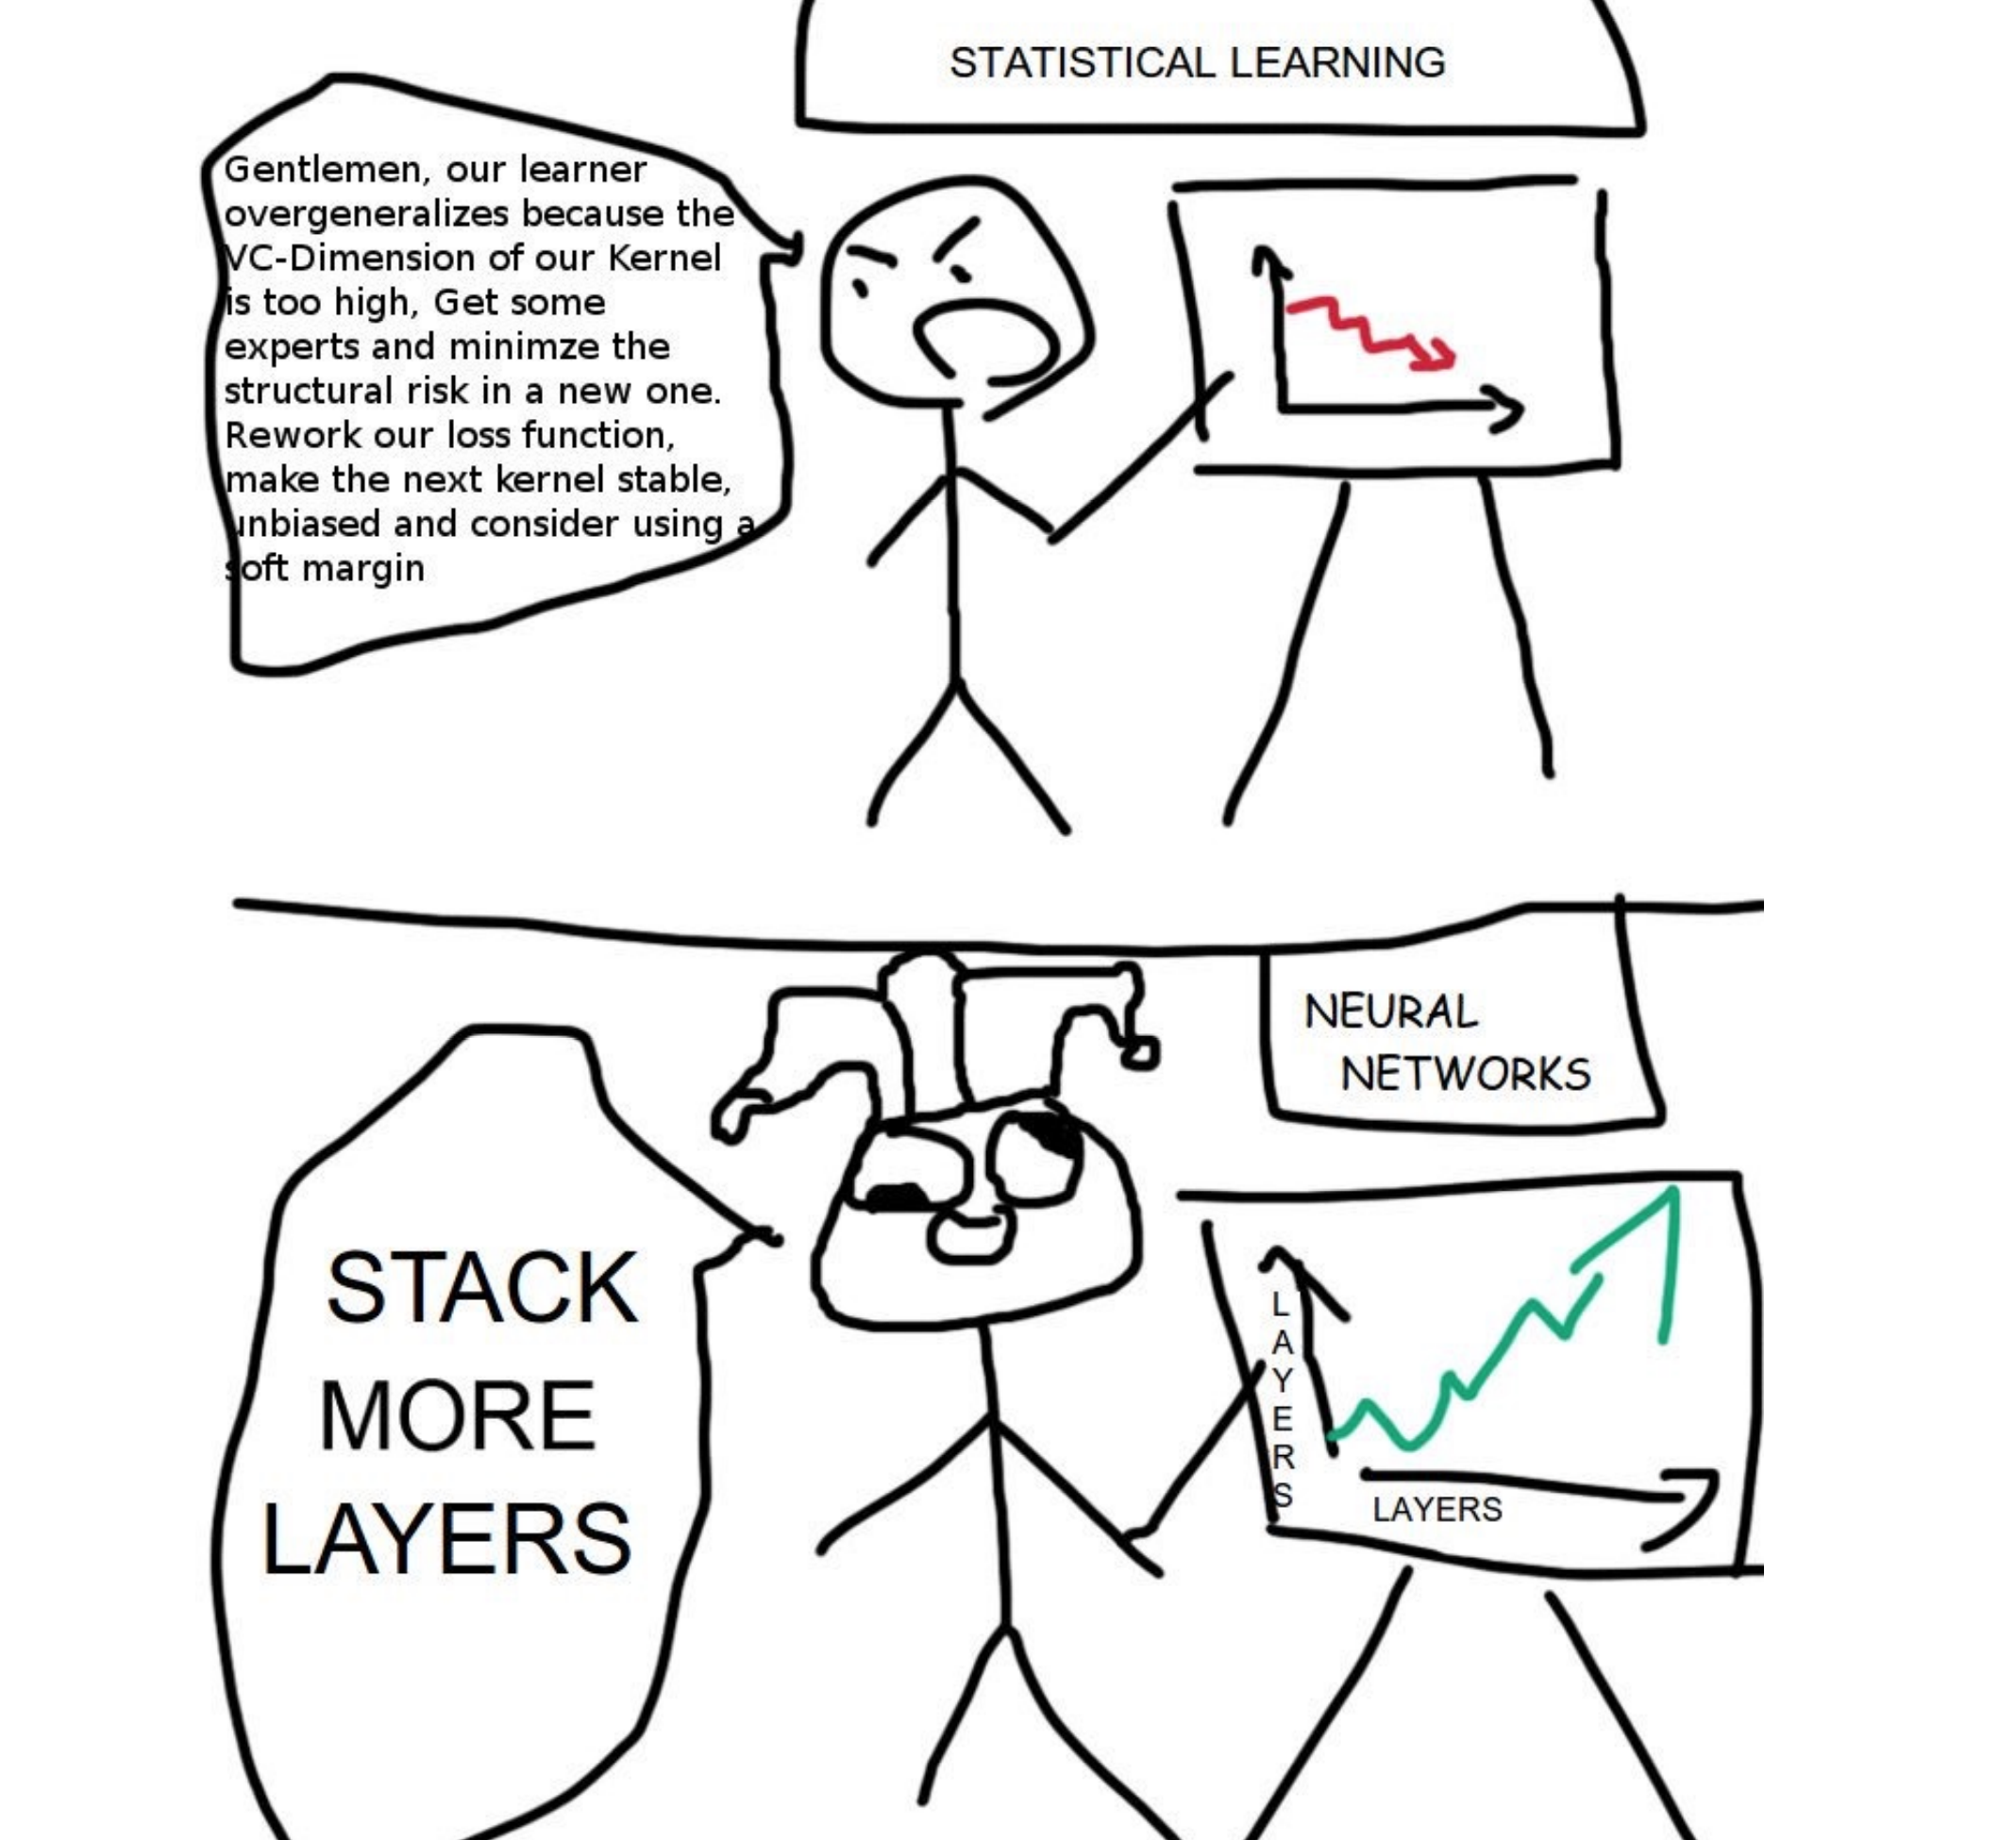
\includegraphics[scale=0.25]{stack_more_layers.png}
    \caption{Good advice from the internet}
    \label{fig:good_advice}
\end{figure}

In this spirit, we ran our model with the following settings:
\begin{figure}[h]
    \centering
    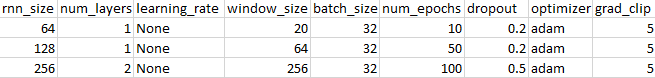
\includegraphics[scale=0.8]{experiment_schedule_2.png}
    \caption{Experiment Schedule}
    \label{fig:experiment_schedule1}
\end{figure}

\section{Results}
All trained models can be found in the folder \textit{experiments}. Each model contains a subfolder \textit{generated} with a \textit{.mid} file containing model generated output using the song "In the year 2525" (not part of the training dataset).


\end{document}
